\documentclass[14pt]{extbook}
\usepackage{multicol, enumerate, enumitem, hyperref, color, soul, setspace, parskip, fancyhdr} %General Packages
\usepackage{amssymb, amsthm, amsmath, latexsym, units, mathtools} %Math Packages
\everymath{\displaystyle} %All math in Display Style
% Packages with additional options
\usepackage[headsep=0.5cm,headheight=12pt, left=1 in,right= 1 in,top= 1 in,bottom= 1 in]{geometry}
\usepackage[usenames,dvipsnames]{xcolor}
\usepackage{dashrule}  % Package to use the command below to create lines between items
\newcommand{\litem}[1]{\item#1\hspace*{-1cm}\rule{\textwidth}{0.4pt}}
\pagestyle{fancy}
\lhead{Makeup Progress Quiz 3}
\chead{}
\rhead{Version ALL}
\lfoot{1648-1753}
\cfoot{}
\rfoot{Summer C 2021}
\begin{document}

\begin{enumerate}
\litem{
Solve the equation below. Then, choose the interval that contains the solution.\[ -9(3x + 11) = -5(17x + 8) \]\begin{enumerate}[label=\Alph*.]
\item \( x \in [-2.21, -0.44] \)
\item \( x \in [-3.27, -2.12] \)
\item \( x \in [2.39, 2.83] \)
\item \( x \in [0.73, 2.04] \)
\item \( \text{There are no real solutions.} \)

\end{enumerate} }
\litem{
Find the equation of the line described below. Write the linear equation in the form $ y=mx+b $ and choose the intervals that contain $m$ and $b$.\[ \text{Perpendicular to } 6 x - 7 y = 6 \text{ and passing through the point } (-5, 4). \]\begin{enumerate}[label=\Alph*.]
\item \( m \in [-2.54, -0.89] \hspace*{3mm} b \in [8.92, 9.19] \)
\item \( m \in [-2.54, -0.89] \hspace*{3mm} b \in [1.36, 2.36] \)
\item \( m \in [-2.54, -0.89] \hspace*{3mm} b \in [-2.49, -1.7] \)
\item \( m \in [0.1, 2.72] \hspace*{3mm} b \in [9.7, 10.7] \)
\item \( m \in [-0.93, -0.21] \hspace*{3mm} b \in [-2.49, -1.7] \)

\end{enumerate} }
\litem{
Find the equation of the line described below. Write the linear equation in the form $ y=mx+b $ and choose the intervals that contain $m$ and $b$.\[ \text{Perpendicular to } 8 x - 5 y = 6 \text{ and passing through the point } (7, -9). \]\begin{enumerate}[label=\Alph*.]
\item \( m \in [0.59, 0.76] \hspace*{3mm} b \in [-14.38, -10.38] \)
\item \( m \in [-0.9, -0.3] \hspace*{3mm} b \in [-20, -14] \)
\item \( m \in [-0.9, -0.3] \hspace*{3mm} b \in [-8.62, -3.62] \)
\item \( m \in [-0.9, -0.3] \hspace*{3mm} b \in [1.62, 9.62] \)
\item \( m \in [-1.83, -0.92] \hspace*{3mm} b \in [-8.62, -3.62] \)

\end{enumerate} }
\litem{
Write the equation of the line in the graph below in Standard Form $Ax+By=C$. Then, choose the intervals that contain $A, B, \text{ and } C$.
\begin{center}
    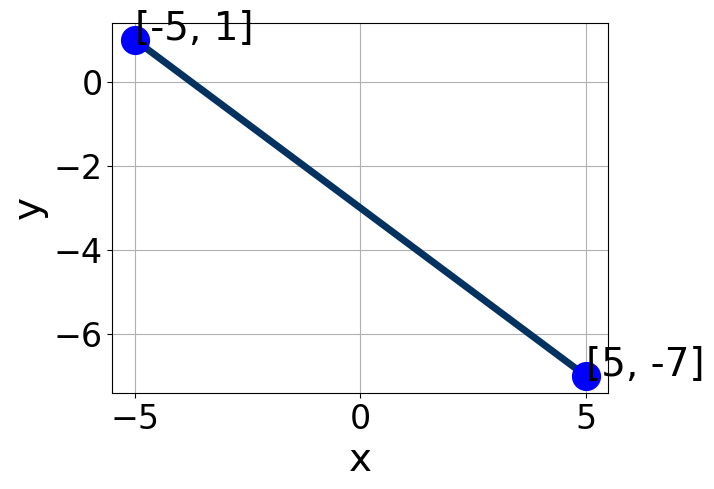
\includegraphics[width=0.5\textwidth]{../Figures/linearGraphToStandardCopyA.png}
\end{center}
\begin{enumerate}[label=\Alph*.]
\item \( A \in [1.8, 6.1], \hspace{3mm} B \in [5, 10], \text{ and } \hspace{3mm} C \in [-17, -7] \)
\item \( A \in [-1.9, 2.9], \hspace{3mm} B \in [1, 3], \text{ and } \hspace{3mm} C \in [-3, -1] \)
\item \( A \in [-1.9, 2.9], \hspace{3mm} B \in [-3, 0], \text{ and } \hspace{3mm} C \in [1, 6] \)
\item \( A \in [1.8, 6.1], \hspace{3mm} B \in [-9, -4], \text{ and } \hspace{3mm} C \in [10, 18] \)
\item \( A \in [-4.1, -2.3], \hspace{3mm} B \in [-9, -4], \text{ and } \hspace{3mm} C \in [10, 18] \)

\end{enumerate} }
\litem{
Solve the linear equation below. Then, choose the interval that contains the solution.\[ \frac{4x + 6}{3} - \frac{7x + 7}{2} = \frac{-7x -3}{8} \]\begin{enumerate}[label=\Alph*.]
\item \( x \in [-1.7, -0.1] \)
\item \( x \in [1, 2.1] \)
\item \( x \in [0.1, 0.6] \)
\item \( x \in [3.8, 5.3] \)
\item \( \text{There are no real solutions.} \)

\end{enumerate} }
\litem{
First, find the equation of the line containing the two points below. Then, write the equation in the form $ y=mx+b $ and choose the intervals that contain $m$ and $b$.\[ (-4, -9) \text{ and } (-6, 11) \]\begin{enumerate}[label=\Alph*.]
\item \( m \in [-11, -7] \hspace*{3mm} b \in [-59, -45] \)
\item \( m \in [-11, -7] \hspace*{3mm} b \in [-8, 2] \)
\item \( m \in [-11, -7] \hspace*{3mm} b \in [48, 58] \)
\item \( m \in [9, 16] \hspace*{3mm} b \in [69, 76] \)
\item \( m \in [-11, -7] \hspace*{3mm} b \in [15, 23] \)

\end{enumerate} }
\litem{
Write the equation of the line in the graph below in Standard Form $Ax+By=C$. Then, choose the intervals that contain $A, B, \text{ and } C$.
\begin{center}
    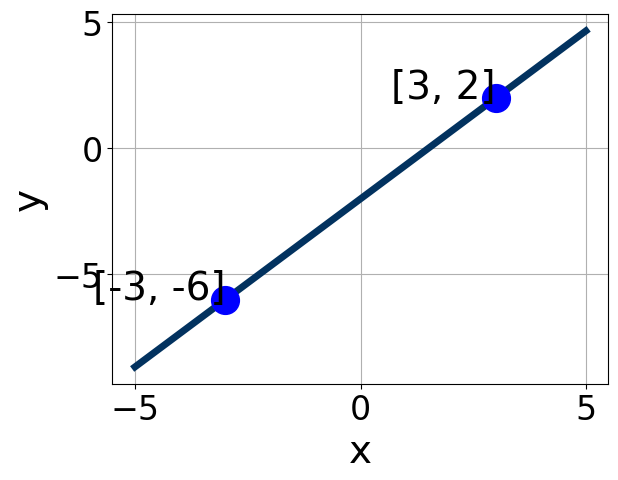
\includegraphics[width=0.5\textwidth]{../Figures/linearGraphToStandardA.png}
\end{center}
\begin{enumerate}[label=\Alph*.]
\item \( A \in [-2.8, 0.3], \hspace{3mm} B \in [-1.56, -0.72], \text{ and } \hspace{3mm} C \in [1.9, 5.3] \)
\item \( A \in [-2.8, 0.3], \hspace{3mm} B \in [-0.23, 1.48], \text{ and } \hspace{3mm} C \in [-4.6, -0.6] \)
\item \( A \in [-5.5, -1.4], \hspace{3mm} B \in [1.28, 4.39], \text{ and } \hspace{3mm} C \in [-7.8, -5.5] \)
\item \( A \in [1.5, 5.9], \hspace{3mm} B \in [-4.02, -2.82], \text{ and } \hspace{3mm} C \in [5.5, 8.2] \)
\item \( A \in [1.5, 5.9], \hspace{3mm} B \in [1.28, 4.39], \text{ and } \hspace{3mm} C \in [-7.8, -5.5] \)

\end{enumerate} }
\litem{
Solve the equation below. Then, choose the interval that contains the solution.\[ -18(3x + 7) = -17(10x + 13) \]\begin{enumerate}[label=\Alph*.]
\item \( x \in [-3.46, -2.92] \)
\item \( x \in [-1.84, -0.97] \)
\item \( x \in [-1.35, -0.48] \)
\item \( x \in [2.86, 3.64] \)
\item \( \text{There are no real solutions.} \)

\end{enumerate} }
\litem{
First, find the equation of the line containing the two points below. Then, write the equation in the form $ y=mx+b $ and choose the intervals that contain $m$ and $b$.\[ (-3, -4) \text{ and } (4, 6) \]\begin{enumerate}[label=\Alph*.]
\item \( m \in [1.1, 4.2] \hspace*{3mm} b \in [-1.52, -0.75] \)
\item \( m \in [1.1, 4.2] \hspace*{3mm} b \in [-0.47, -0.2] \)
\item \( m \in [1.1, 4.2] \hspace*{3mm} b \in [1.45, 2.09] \)
\item \( m \in [-4.7, 1.2] \hspace*{3mm} b \in [11.62, 11.75] \)
\item \( m \in [1.1, 4.2] \hspace*{3mm} b \in [0, 0.79] \)

\end{enumerate} }
\litem{
Solve the linear equation below. Then, choose the interval that contains the solution.\[ \frac{-3x + 5}{3} - \frac{8x + 8}{7} = \frac{-5x + 7}{4} \]\begin{enumerate}[label=\Alph*.]
\item \( x \in [-0.5, 0.1] \)
\item \( x \in [-11.5, -10.9] \)
\item \( x \in [0.9, 1.9] \)
\item \( x \in [-3.1, -1] \)
\item \( \text{There are no real solutions.} \)

\end{enumerate} }
\litem{
Solve the equation below. Then, choose the interval that contains the solution.\[ -5(-12x -6) = -15(14x -4) \]\begin{enumerate}[label=\Alph*.]
\item \( x \in [-0.38, -0.32] \)
\item \( x \in [0.5, 1.22] \)
\item \( x \in [0.25, 0.44] \)
\item \( x \in [-0.08, 0.22] \)
\item \( \text{There are no real solutions.} \)

\end{enumerate} }
\litem{
Find the equation of the line described below. Write the linear equation in the form $ y=mx+b $ and choose the intervals that contain $m$ and $b$.\[ \text{Perpendicular to } 3 x - 7 y = 6 \text{ and passing through the point } (-4, -4). \]\begin{enumerate}[label=\Alph*.]
\item \( m \in [-2.6, -1.6] \hspace*{3mm} b \in [-18.33, -11.33] \)
\item \( m \in [1.4, 3.4] \hspace*{3mm} b \in [4.33, 13.33] \)
\item \( m \in [-1.3, 0.6] \hspace*{3mm} b \in [-18.33, -11.33] \)
\item \( m \in [-2.6, -1.6] \hspace*{3mm} b \in [-3, 3] \)
\item \( m \in [-2.6, -1.6] \hspace*{3mm} b \in [9.33, 15.33] \)

\end{enumerate} }
\litem{
Find the equation of the line described below. Write the linear equation in the form $ y=mx+b $ and choose the intervals that contain $m$ and $b$.\[ \text{Parallel to } 5 x + 7 y = 11 \text{ and passing through the point } (-8, -5). \]\begin{enumerate}[label=\Alph*.]
\item \( m \in [0.26, 1.53] \hspace*{3mm} b \in [-1.3, 2.8] \)
\item \( m \in [-2.29, -0.89] \hspace*{3mm} b \in [-13.3, -9.8] \)
\item \( m \in [-0.83, -0.61] \hspace*{3mm} b \in [9.8, 10.9] \)
\item \( m \in [-0.83, -0.61] \hspace*{3mm} b \in [1.3, 3.8] \)
\item \( m \in [-0.83, -0.61] \hspace*{3mm} b \in [-13.3, -9.8] \)

\end{enumerate} }
\litem{
Write the equation of the line in the graph below in Standard Form $Ax+By=C$. Then, choose the intervals that contain $A, B, \text{ and } C$.
\begin{center}
    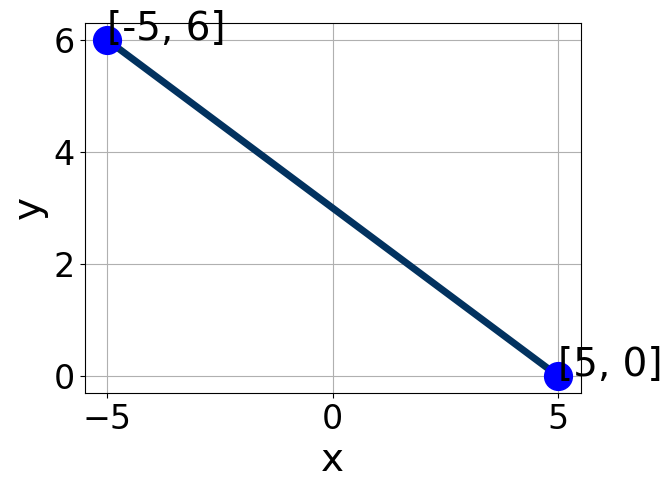
\includegraphics[width=0.5\textwidth]{../Figures/linearGraphToStandardCopyB.png}
\end{center}
\begin{enumerate}[label=\Alph*.]
\item \( A \in [1.1, 6.7], \hspace{3mm} B \in [4, 8], \text{ and } \hspace{3mm} C \in [14, 21] \)
\item \( A \in [0.4, 0.8], \hspace{3mm} B \in [1, 3], \text{ and } \hspace{3mm} C \in [3, 6] \)
\item \( A \in [1.1, 6.7], \hspace{3mm} B \in [-8, -4], \text{ and } \hspace{3mm} C \in [-16, -13] \)
\item \( A \in [-5.2, 0.2], \hspace{3mm} B \in [-8, -4], \text{ and } \hspace{3mm} C \in [-16, -13] \)
\item \( A \in [0.4, 0.8], \hspace{3mm} B \in [-4, 0], \text{ and } \hspace{3mm} C \in [-3, -2] \)

\end{enumerate} }
\litem{
Solve the linear equation below. Then, choose the interval that contains the solution.\[ \frac{7x -8}{5} - \frac{-4x -7}{3} = \frac{6x -9}{4} \]\begin{enumerate}[label=\Alph*.]
\item \( x \in [-0.5, 2.8] \)
\item \( x \in [-8.1, -5.8] \)
\item \( x \in [-1.1, 1.1] \)
\item \( x \in [-3.4, -1] \)
\item \( \text{There are no real solutions.} \)

\end{enumerate} }
\litem{
First, find the equation of the line containing the two points below. Then, write the equation in the form $ y=mx+b $ and choose the intervals that contain $m$ and $b$.\[ (-4, -6) \text{ and } (8, -11) \]\begin{enumerate}[label=\Alph*.]
\item \( m \in [-2.9, 0.3] \hspace*{3mm} b \in [-3.5, 0.2] \)
\item \( m \in [-2.9, 0.3] \hspace*{3mm} b \in [6.7, 8.3] \)
\item \( m \in [-0.4, 1] \hspace*{3mm} b \in [-17, -13.7] \)
\item \( m \in [-2.9, 0.3] \hspace*{3mm} b \in [-22.3, -17] \)
\item \( m \in [-2.9, 0.3] \hspace*{3mm} b \in [-8.4, -6.1] \)

\end{enumerate} }
\litem{
Write the equation of the line in the graph below in Standard Form $Ax+By=C$. Then, choose the intervals that contain $A, B, \text{ and } C$.
\begin{center}
    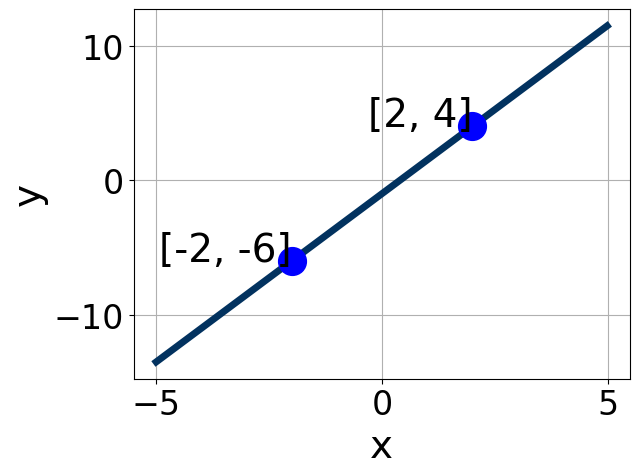
\includegraphics[width=0.5\textwidth]{../Figures/linearGraphToStandardB.png}
\end{center}
\begin{enumerate}[label=\Alph*.]
\item \( A \in [1.2, 7.5], \hspace{3mm} B \in [-2.09, -1.98], \text{ and } \hspace{3mm} C \in [1.77, 2.7] \)
\item \( A \in [-8.3, -4.3], \hspace{3mm} B \in [1.68, 2.11], \text{ and } \hspace{3mm} C \in [-2.34, -1.66] \)
\item \( A \in [-3.3, -2], \hspace{3mm} B \in [0.56, 1.64], \text{ and } \hspace{3mm} C \in [-1.47, 0.03] \)
\item \( A \in [1.2, 7.5], \hspace{3mm} B \in [1.68, 2.11], \text{ and } \hspace{3mm} C \in [-2.34, -1.66] \)
\item \( A \in [-3.3, -2], \hspace{3mm} B \in [-1.39, -0.82], \text{ and } \hspace{3mm} C \in [0.25, 1.12] \)

\end{enumerate} }
\litem{
Solve the equation below. Then, choose the interval that contains the solution.\[ -15(-9x -12) = -4(-18x -17) \]\begin{enumerate}[label=\Alph*.]
\item \( x \in [3.66, 4.21] \)
\item \( x \in [-4.56, -3.75] \)
\item \( x \in [-2.55, -1.28] \)
\item \( x \in [-1.65, 0.08] \)
\item \( \text{There are no real solutions.} \)

\end{enumerate} }
\litem{
First, find the equation of the line containing the two points below. Then, write the equation in the form $ y=mx+b $ and choose the intervals that contain $m$ and $b$.\[ (11, 2) \text{ and } (9, -11) \]\begin{enumerate}[label=\Alph*.]
\item \( m \in [4.5, 8.5] \hspace*{3mm} b \in [-74.5, -67.5] \)
\item \( m \in [-14.5, -4.5] \hspace*{3mm} b \in [46.5, 50.5] \)
\item \( m \in [4.5, 8.5] \hspace*{3mm} b \in [-15, -6] \)
\item \( m \in [4.5, 8.5] \hspace*{3mm} b \in [-20, -17] \)
\item \( m \in [4.5, 8.5] \hspace*{3mm} b \in [65.5, 71.5] \)

\end{enumerate} }
\litem{
Solve the linear equation below. Then, choose the interval that contains the solution.\[ \frac{-5x + 4}{7} - \frac{6x -3}{5} = \frac{-7x -4}{4} \]\begin{enumerate}[label=\Alph*.]
\item \( x \in [11.22, 16.22] \)
\item \( x \in [65.96, 67.96] \)
\item \( x \in [4.91, 8.91] \)
\item \( x \in [0.54, 1.54] \)
\item \( \text{There are no real solutions.} \)

\end{enumerate} }
\litem{
Solve the equation below. Then, choose the interval that contains the solution.\[ -17(-12x + 3) = -18(7x -14) \]\begin{enumerate}[label=\Alph*.]
\item \( x \in [-1.29, -0.35] \)
\item \( x \in [0.2, 0.65] \)
\item \( x \in [-3.56, -1.75] \)
\item \( x \in [0.83, 1.17] \)
\item \( \text{There are no real solutions.} \)

\end{enumerate} }
\litem{
Find the equation of the line described below. Write the linear equation in the form $ y=mx+b $ and choose the intervals that contain $m$ and $b$.\[ \text{Parallel to } 3 x - 4 y = 12 \text{ and passing through the point } (6, 9). \]\begin{enumerate}[label=\Alph*.]
\item \( m \in [0.67, 1.16] \hspace*{3mm} b \in [4.47, 5.43] \)
\item \( m \in [1.31, 1.56] \hspace*{3mm} b \in [4.47, 5.43] \)
\item \( m \in [-0.91, -0.16] \hspace*{3mm} b \in [12.68, 13.77] \)
\item \( m \in [0.67, 1.16] \hspace*{3mm} b \in [-5.48, -3.1] \)
\item \( m \in [0.67, 1.16] \hspace*{3mm} b \in [2.96, 3.8] \)

\end{enumerate} }
\litem{
Find the equation of the line described below. Write the linear equation in the form $ y=mx+b $ and choose the intervals that contain $m$ and $b$.\[ \text{Perpendicular to } 6 x - 7 y = 7 \text{ and passing through the point } (-6, -8). \]\begin{enumerate}[label=\Alph*.]
\item \( m \in [-0.99, -0.1] \hspace*{3mm} b \in [-15.17, -14.25] \)
\item \( m \in [-1.91, -1.14] \hspace*{3mm} b \in [-15.17, -14.25] \)
\item \( m \in [-1.91, -1.14] \hspace*{3mm} b \in [-4.17, -1.8] \)
\item \( m \in [0.93, 1.7] \hspace*{3mm} b \in [-1.39, -0.24] \)
\item \( m \in [-1.91, -1.14] \hspace*{3mm} b \in [14.93, 15.47] \)

\end{enumerate} }
\litem{
Write the equation of the line in the graph below in Standard Form $Ax+By=C$. Then, choose the intervals that contain $A, B, \text{ and } C$.
\begin{center}
    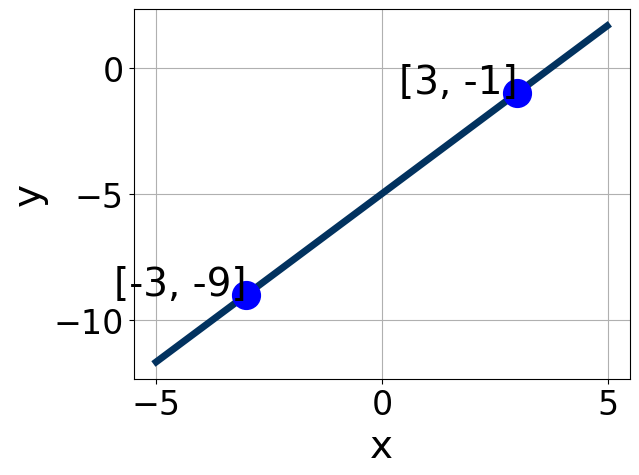
\includegraphics[width=0.5\textwidth]{../Figures/linearGraphToStandardCopyC.png}
\end{center}
\begin{enumerate}[label=\Alph*.]
\item \( A \in [-2.9, -0.3], \hspace{3mm} B \in [0.01, 1.56], \text{ and } \hspace{3mm} C \in [-6, -2] \)
\item \( A \in [-7, -1.8], \hspace{3mm} B \in [2.87, 3.77], \text{ and } \hspace{3mm} C \in [-16, -6] \)
\item \( A \in [0, 4.8], \hspace{3mm} B \in [2.87, 3.77], \text{ and } \hspace{3mm} C \in [-16, -6] \)
\item \( A \in [0, 4.8], \hspace{3mm} B \in [-3.02, -2.9], \text{ and } \hspace{3mm} C \in [10, 20] \)
\item \( A \in [-2.9, -0.3], \hspace{3mm} B \in [-1.54, -0.99], \text{ and } \hspace{3mm} C \in [4, 11] \)

\end{enumerate} }
\litem{
Solve the linear equation below. Then, choose the interval that contains the solution.\[ \frac{-8x + 7}{4} - \frac{-5x + 3}{7} = \frac{-6x -5}{8} \]\begin{enumerate}[label=\Alph*.]
\item \( x \in [-0.65, 0.35] \)
\item \( x \in [14.8, 21.8] \)
\item \( x \in [3.63, 4.63] \)
\item \( x \in [4.23, 6.23] \)
\item \( \text{There are no real solutions.} \)

\end{enumerate} }
\litem{
First, find the equation of the line containing the two points below. Then, write the equation in the form $ y=mx+b $ and choose the intervals that contain $m$ and $b$.\[ (9, 5) \text{ and } (-11, -8) \]\begin{enumerate}[label=\Alph*.]
\item \( m \in [-0.1, 2.1] \hspace*{3mm} b \in [0.2, 0.9] \)
\item \( m \in [-0.1, 2.1] \hspace*{3mm} b \in [1, 5.7] \)
\item \( m \in [-1.4, 0.2] \hspace*{3mm} b \in [-17.6, -13.7] \)
\item \( m \in [-0.1, 2.1] \hspace*{3mm} b \in [-1.3, 0.7] \)
\item \( m \in [-0.1, 2.1] \hspace*{3mm} b \in [-4.3, -2.4] \)

\end{enumerate} }
\litem{
Write the equation of the line in the graph below in Standard Form $Ax+By=C$. Then, choose the intervals that contain $A, B, \text{ and } C$.
\begin{center}
    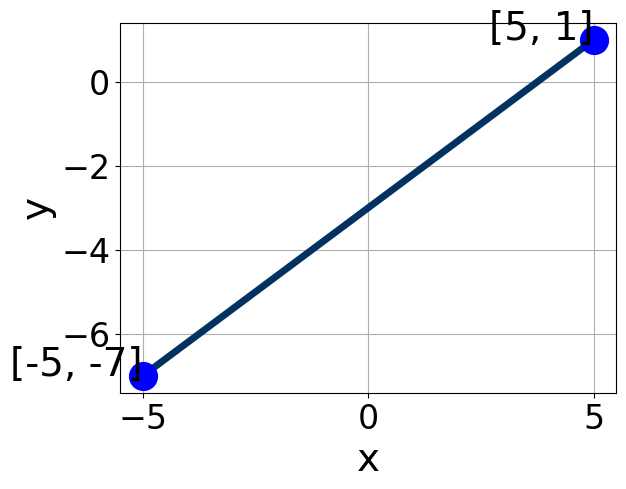
\includegraphics[width=0.5\textwidth]{../Figures/linearGraphToStandardC.png}
\end{center}
\begin{enumerate}[label=\Alph*.]
\item \( A \in [3.8, 4.4], \hspace{3mm} B \in [2.3, 8.6], \text{ and } \hspace{3mm} C \in [-16, -8] \)
\item \( A \in [-3, 0.6], \hspace{3mm} B \in [-1.8, -0.4], \text{ and } \hspace{3mm} C \in [1, 4] \)
\item \( A \in [-3, 0.6], \hspace{3mm} B \in [-0.4, 2.2], \text{ and } \hspace{3mm} C \in [-6, -1] \)
\item \( A \in [-5.7, -3.3], \hspace{3mm} B \in [2.3, 8.6], \text{ and } \hspace{3mm} C \in [-16, -8] \)
\item \( A \in [3.8, 4.4], \hspace{3mm} B \in [-5.3, -3.5], \text{ and } \hspace{3mm} C \in [13, 20] \)

\end{enumerate} }
\litem{
Solve the equation below. Then, choose the interval that contains the solution.\[ -10(8x + 5) = -14(7x + 9) \]\begin{enumerate}[label=\Alph*.]
\item \( x \in [-5.22, -2.22] \)
\item \( x \in [5.78, 10.78] \)
\item \( x \in [-0.99, 3.01] \)
\item \( x \in [-9.78, -6.78] \)
\item \( \text{There are no real solutions.} \)

\end{enumerate} }
\litem{
First, find the equation of the line containing the two points below. Then, write the equation in the form $ y=mx+b $ and choose the intervals that contain $m$ and $b$.\[ (11, 4) \text{ and } (7, -11) \]\begin{enumerate}[label=\Alph*.]
\item \( m \in [3.75, 8.75] \hspace*{3mm} b \in [-42.25, -33.25] \)
\item \( m \in [-8.75, -1.75] \hspace*{3mm} b \in [7.25, 21.25] \)
\item \( m \in [3.75, 8.75] \hspace*{3mm} b \in [-12, 0] \)
\item \( m \in [3.75, 8.75] \hspace*{3mm} b \in [33.25, 42.25] \)
\item \( m \in [3.75, 8.75] \hspace*{3mm} b \in [-23, -16] \)

\end{enumerate} }
\litem{
Solve the linear equation below. Then, choose the interval that contains the solution.\[ \frac{4x -9}{7} - \frac{7x -9}{4} = \frac{-4x -5}{6} \]\begin{enumerate}[label=\Alph*.]
\item \( x \in [-8.28, -2.28] \)
\item \( x \in [1.51, 5.51] \)
\item \( x \in [-3.8, -0.8] \)
\item \( x \in [8.77, 10.77] \)
\item \( \text{There are no real solutions.} \)

\end{enumerate} }
\end{enumerate}

\end{document}